\begin{beispiel}[Logistisches Wachstum (gebremst)]
\mbox{}\\
$u(t) $ sei Größe einer Population.
Berücksichtige hemmende Faktoren (beschränkte Resourcen, Krankheiten, Kriege,...)

\textbf{Modellannahme:} wegen beschränkter Kapazität kann $u(t) $
eine gewisse Maximalgröße $M$ nicht überschrieten und
$\Delta u $ ist proportional zu $u, \ M-u, \ \Delta t \\
\Rightarrow \Delta u = \alpha u(M-u) \Delta t 
\xRightarrow{\text{wie oben}} 
u' = \gamma u - \tau u^2 (\gamma = \alpha M, \ \tau = \alpha $\\
Interpretation: Wachstum $u$ wird durch Term $-\tau u^2 $ für große $u$ 
stärker gebremst als für kleine $u$. \\

Allgemeine Lösung: für $u(0) = u_0 \\
u(t) = \frac{\gamma}{\tau + \left(\frac{\gamma}{u_0} - \tau \right) e^{-\gamma t}}
= \frac{M}{1+\left(\frac{M}{u_0} - 1 \right) e^{-\gamma M t}} $ \\
Sei  $\alpha, M > 0 \Rightarrow u(t) \xrightarrow{t\rightarrow\infty} M $\\
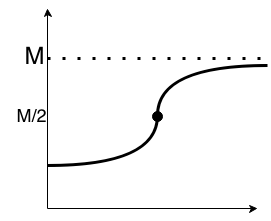
\includegraphics[scale=0.5]{pictures/011-01.png}\\                            
$u_0 \in (0,M)\\
u_0 >M\\
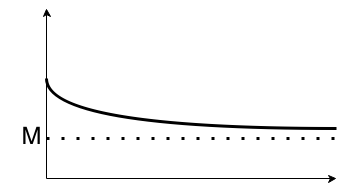
\includegraphics[scale=0.5]{pictures/011-02.png}\\
u_0 = M \Rightarrow u(t) = M \forall t $\\

Insbesondere beschreibt logistisches Wachstum:
\begin{itemize}
    \item Gewichtszunahme
    \item Höhenwachstum von Sonnenblumen
    \item Verbreitung von Gerüchten
\end{itemize}

\end{beispiel}

\begin{beispiel}[Freier Fall]

$v(t) = u'(t) $ Geschwindigkeit\\

\textbf{Modellannahme:} Newtonsches Kraftgesetz: $K = m u'' $\\
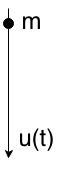
\includegraphics[scale=0.5]{pictures/011-03.png}\\                            
Schwerkraft nahe Erdoberfläche $K = mg$ ($g$ - 'Gravitationskonstante')\\
$\Rightarrow u'' = g $ bzw. $v' = g \\
\Rightarrow v(t) = v_0 + gt \\
\Rightarrow u(t) = u_0 + v_0 t + \frac{1}{2} g t^2 $\\
Offenbar liefert Vorgabe von $u(0) = u_0 $ und $u'(0) = v_0 $ eine eindeutige Lösung
der Differenzialgleichung (Anfangswertproblem).\\
Alternativ könnte man $u(0) = u_0 $ und $u(t_1) = u_1 $ vorschreiben:\\
$\Rightarrow u_1 = u_0 + v_0 t_1 + \frac{1}{2} g t_1^2 \\
\Rightarrow v_0 = \frac{u_1 - u_0 - \frac{1}{2} g t_1^2}{t_1} $\\
das heißt man erhält wieder eine eindeutige Lösung (Randwertproblem).
\end{beispiel}

\textbf{Wichtige Fragestellungen bei Behandlung von Differenzialgleichungen}\\
\begin{itemize}
    \item \emph{Existenz einer Lösung}
        \begin{itemize}
            \item explizite Lösungen findet man nur in einigen Spezialfällen\\
                ($\rightarrow $ Näherungslösung mittels Computer)
            \item 
                \emph{aber} Existenz einer Lösung kann 
                sehr allgemein abstrakt gezeigt werden (zumindest lokal)
        \end{itemize}
        $\Rightarrow $\emph{qualitative Untersuchungen} 
        der nicht explizit bekannten Lösungen spielen eine wichtige Rolle,
        zum Beispiel:
        \begin{itemize}
            \item Fortsetzunge
            \item Asymptotisches Verhalten
            \item Stabilität
            \item Regularität
            \item Periodizität
            \item ...
        \end{itemize}
    \item \emph{Eindeutigkeit einer Lösung}
        \begin{itemize}
            \item obige Beispiele zeigen, dass idR Parameter auftreten,
                 woraus unendlich viele Lösungen folgen
            \item durch Vorgabe von geeigneten Anfangswerten $(u(0), \ u'(0), \ldots)$
                bzw. von geeigneten  Randwerten $(u(t_0) = u_0, (u(t_1) = u_1) $ 
                ergibt sich häufig eine  eindeutige Lösung
            \item manche Probleme haben in natürlicher Weise keine eindeutige Lösung,
                z.B. Beulprobleme
        \end{itemize}
    \item \emph{Stetige Abhängigkeit der Lösung von Parametern} \\
        Parameter = Anfangswerte, Koeffizienten\\
        Problem: Parameter sind nie exakt messbar! Geringfügige Abweichungen können
        in (chaotischen) Systeme zu völlig unterschiedlichen Lösungen führen 
        (z.B. Doppelpendel). \\
        'Das ist eine ganz wichtige Sache, muss man wissen!'\\
        $\Rightarrow $ kleine Störung der Parameter sollten nur 
        kleine Veränderung der Lösung bewirken, d.h. die Lösung sollte stetig
        von den Parametern abhängen.
\end{itemize}

\begin{definition}[Korrekte Problemstellung]
Man sagt ein Problem ist \textbf{korrekt gestellt} falls die Lösung:
\begin{itemize}
    \item existiert,
    \item eindeutig ist,
    \item stetig von den Parametern abhängt.
\end{itemize}
\end{definition}

Literatur:\\
Walter: Gewöhnliche Differenzialgleichungen, Springer\\
Heuser: Gewöhnliche Differenzialgleichungen

\section{Differentialgleichungen 1. Ordnung}

Allgemeine Form: $f(x, u(x), u'(x)) = 0 $

\subsection{Explizite Dgl. 1. Ordnung - Elementar integrierbare Fälle}

Allgemeine explizite Dgl. 1. Ordnung:
$u'8x) = f(x, u(x)) $

Annahme: $f: D \subset \mathbb{R}^2 \rightarrow \mathbb{R} $ stetig
($\mathbb{R}^2 \leftrightarrow (x,u)$-Ebene)

Lösungsbegriff:
Sei $I \subset \mathbb{R} $ Intervall\\
Funktion $u: I \subset \mathbb{R} \rightarrow R $ ist Lösung der Dgl. falls
$u$ auf $I$ diffferenzierbar,\\
$(x, u(x)) \in D \ \forall x \in I $ und $u'(x) = f(x, u(x)) $ ist.

\begin{enumerate}
    \item[i)] \emph{Vorbemerkung: Richtungsfeld, Polygonzug:} $u'(x) = f(x, u(x))$\\
        Sei $u$ Lösung mit $(\tilde{x}, u(\tilde{x})) = (\tilde{x}, \tilde{u}) \in D\\
        \Rightarrow f((\tilde{x}, \tilde{u}) $ gibt Anstieg der Kurve $u(.) $ in $x$\\
        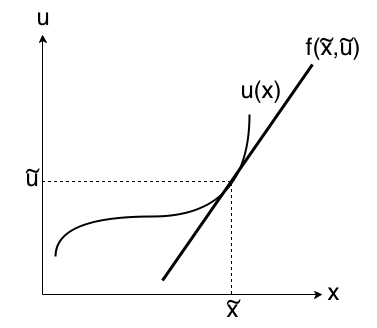
\includegraphics[scale=0.5]{pictures/011-04.png}\\
        $(x, u, f(x,u)) $ heißt \emph{Richtungsfeld}
        ohne(!) Kenntnis der Umgebung gibt es Anstieg von $u(.)$ in $x$ 
        für den Fall, dass $(x,u) $ zum Graphen von $u(.) $ gehört.\\
        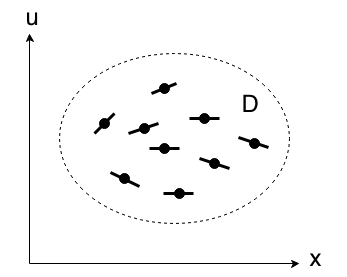
\includegraphics[scale=0.5]{pictures/011-05.png}\\
        \emph{Problem:} suche Kurve $u(.) $ die zum Richtungsfeld passt.\\
        \emph{Anfangsgswert:} In 'vielen Fällen' geht durch jeden Punkt $(x,u) \in D $
        genau eine Kurve \\
        $\Rightarrow $ Vorgabe von $(x_0, u_0) = (x_0, u(x_0)) $ 
        liefert eindeutige Lösung
        
        \emph{Näherungslösung:} Polygonzug\\
        wähle $x_k = x_0 + k h, \ k= 1 \ldots n, \ h$ - Schrittweite\\
        $u_0 = u(x_0) $wird als AW vorgegeben.\\
        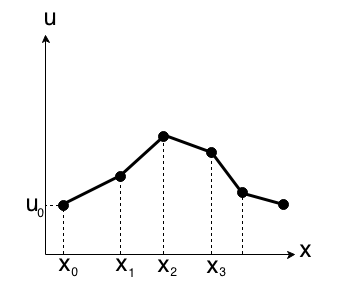
\includegraphics[scale=0.5]{pictures/011-06.png}\\                    
        Schrittweise setzt man $u_k = u_{k+1} + h f(x_{k-1}, u_{k-1}), \ k= 1 \ldots n $\\
        in 'vielen Fällen' konvergiert Polygonzug für $h \rightarrow 0 $ gegen Lösung.
    \item[ii)]$\mathbf{u'(x) = f(x)}$
        $\Rightarrow  u $ ist Stammfunktion von $f$
        Sei $f$ im Intervall $I \subset \mathbb{R} $ definiert und stetig, $x_0 \in I $\\
        Allgemeine Lösung: (vgl. Grundkurs)\\
        $u(x) = \int\limits_{x_0}^x f(\xi) \mathrm{d}\xi + u_0, \ u_0 \in \mathbb{R} $\\
        Vorgabe $u_0$ entspricht gerade dem AW $u(x_0) = u_0 $
    \item[iii)]$\mathbf{u'(x) = f(x) g(u(x))} $ Dgl. mit getrennten Variablen\\
        \emph{Heuristik:}
        $\diff{u}{x} = f(x) g(u) 
        \Rightarrow  \frac{1}{g(u)} \mathrm{d}u = f(x) \mathrm{d}x $\\
        Integration: $\int \frac{1}{g(u)} \mathrm{d}u = \int f(x) \mathrm{d}x $\\
        um AWP $u(x_0) = u_0 $ zu lösen nehme \\
        $\int\limits_{u_0}^u \frac{1}{g(s)} \mathrm{d}s 
        = \int\limits_{x_0}^x f(x) \mathrm{d}x $\\
        Auflösung nach $u$ liefert Lösung $u = u(x)$
        \begin{beispiel*}
        $u' = e^u \sin x, \ u(x_0) = u_0 \\
        \Rightarrow \int\limits_{u_0}^u e^{-s} \mathrm{d}s
        = \int\limits_{x_0}^x \sin \mathrm{d}t
        \Rightarrow \left[ -e^{-s} \right]_{u_0}^u = \left[ - \cos t \right]_{x_0}^x \\
        \Rightarrow e^{-u} = \cos x - \cos x_0 + e^{-u_0}
        \Rightarrow u(x) = -\ln ( \cos x 
        + \underbrace{e^{-u_0} - \cos x_0}_{\coloneqq c})\\
        $        
        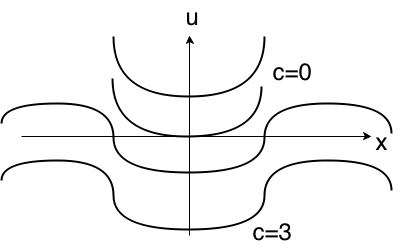
\includegraphics[scale=0.5]{pictures/011-07.png}\\                            
        Es ist zu beachten, das sich abhängig von den AW der Definitionsbereich der
        Lösung ändert.\\
        Probe: $u' = 
        \frac{
        \sin x}
        {\cos x + e^{-u_0} - \cos x_0}
        = e^u \sin x
        $
        \end{beispiel*}        
\end{enumerate}
